\chapter{Compilers}
\graphicspath{ {./images/} }


\textbf{Compilers}\cite{dragonbook} are that piece of software that \textit{translates} the programs in one language to other languages. They are different from \textbf{Assembler}. An assembler converts the assebly codes to final machines' instruction codes according to the ISA of the target computer hardware. Compilers are generally thought to convert higher level programs to low level programs. They are of different types like Cross compilers, Bootstrap Compilers (it comes under cross compilers)
, Transilers and De-compilers. The basic operations carried by most of the compilers are :\\

\section{Lexical Analysis}
This is the first part of any compiler that takes in the program spurce code and does word-substitutions, Macro expansions, generating \textit{Tokens} and cleaning up extra white spaces. All this work is done by using regular expression to increase compactness of input code. The tokens when combined in a special way form what is known as \textbf{Abstract Syantax Trees (AST)}. The regular expressions are interpreted as \textit{Non-Deterministic Finite Automata (NDFA)} since the states or the inner expression in between any two parts of a Regex can't be fixed since it will vary with the input used. Thus the NDFA is converted to \textit{Deterministic Finite Automata (DFA)} which will be parsed to AST using the technique of \textit{$\epsilon$-Transformation}.\\

\section{Syntax Analysis or Parsing}
This is the process of recombining the context-free grammatical tokens into a data structure, syntax tree. It is important that any sort of syntax error should be reported at this point of compilation. Context-free grammar is a recursive notation for describing sets of strings and imposing a structure on each such string \underline{without consiering the context in which the syntax is generated}.\\ 

\subsection{Abstract Syntax Trees and Abstract Binding Trees}
In computer science, an abstract syntax tree (AST), or just syntax tree, is a tree representation of the abstract syntactic structure of source code written in a programming language. It is "Abstract" in the sense that it does not represent every detail appearing in the real syntax of the programming language used, but rather just the structural and content-related details.\\

An abstract syntax tree is an ordered tree whose leaves are variables and whose interior nodes are operators whose arguments are its children. Ast’s are classified into a variety of sorts corresponding to different forms of syntax that divide ASTs into syntactic categories. For example, common programming languages often have a syntactic distinction between commands and an expression. These are two type of sorts for ASTs.\\

\textbf{Abstract Binding Trees (ABT)} enrich the meaning of AST with the methods to introduce new variables and symbols called \textit{bindings} to an existing AST. It should be noted that it is a theoretical concept and \underline{only AST is used in compilers while parsing}. The additions are performed within a given range of significance of the added terms called its \textit{scope}. In desinging type systems, we therefore deal with these ABT to construct new language.\\ 

Writing a new Programming language grammar basically involves writing syntactic sugar for \textit{Expressions, Statements }(often called commands) and \textit{Declaration} like header declarations and variable assisgnments. There are some \textbf{rules} defined and \textit{Judgements and derivations} are performed on them. The derivations are mostly inductive and also covers the finite aspect of machine. This can be understood in a way that DFA is mantained and machine never goes to a NDFA state.\\

For example here is a derivation of successor of a natural number, [ succ(succ(succ(zero)))nat ] : 

\[\dfrac{\dfrac{\dfrac{\dfrac{}{zero\quad nat}}{succ(zero) \quad nat}}{succ(succ(zero)) \quad nat}}{succ(succ(succ(zero))) \quad nat} \] .

The denominator in the expression is an inductive derivation from the numberator conditions.

\section{Type Checking}
This is one of the most important part where data consistency is checked of input source code. The Compiler may exploit or depend on type information, which makes it natural to combine calculation of types with the actual translation of source code. A language is considered to be type-safe if does not allow violation of basic data types. The varying level of strictness leads to formation of weak and strong type safe languages.\\

\begin{figure}[!htb]
\centering
  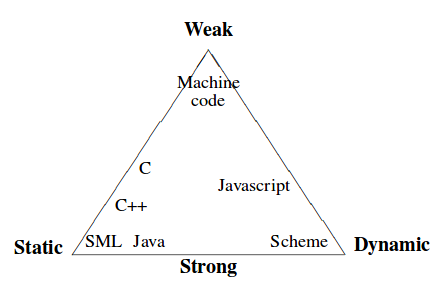
\includegraphics[scale=0.5]{type_check}
  \caption{Design Space of Types (source : Dragon book of compiler Technology)}
\end{figure}

It shows a diagram of the design space of static vs. dynamic and weak vs. strong typing, placing some well-known programming languages in this design space.

\section{Optimization}

This part deals with converting the present code as AST into more efficient using a series of transformations that makes the code use lesser sources but produces same output and variable scope is maintained throughout. Some of the common optimization techniques are :\\

\textbf{Peephole optimizations} replaces a complex multi-step instruction by an instruction of less-number of steps preferably a single step, for example multiplication by 2 is equivalent ot rotating bits to left by 1. \textbf{Data Flow Optimizations} convert expressions into simple to reduce number of duplicate expressions. \textbf{Static Single Assignment (SSA) optimization} involves assigning variables only a single value. If variables have same values then they are considered as one variable only. Scope Tables are used in these cases.

\section{Code Generation}
This part converts the optimized AST into machine codes of a hardware compatible ISA representation. It involves expoliting complex instructions and carefully placing jump and branch instructions for the machine code program. This part is also to be optimized and texhiques of \textit{Register allocation, Instruction selection, Instruction scheduling} and \textit{Rematerialization}. 

\section{Interpreter}
Interpreters are different from the compilers only in the aspect it performs operations as the code is produced without having a previously compiled code and then executing it. It works similar to a compiler in terms of basic steps but uses an \textbf{Interediate Representation (IR)} of AST before producing machine code and executing it too.\\

\textbf{Low Level Virtual Machine (LLVM)}\cite{llvm} is a popular compiler technology that takes into account the benefits of IR in compilation. It is used all over now and has increased portability of softwares a lot. Recently the \textit{Polyhedral Loop Optimizations (Polly)} in the LLVM IR has gained popularity and they have been used in all possible places.\\

